\chapter{Модель \crr}
\label{ch:crr}
\chaptertoc

Модель \crr\ (КРР) "--- это многошаговая биномиальная модель.
В отличие от одношаговой модели, в ней возникает задача динамической репликации, в которой реплицирующий портфель нужно ребалансировать с течением времени.
Модель КРР также интересна тем, что из нее в пределе можно получить известную модель \bs\ (см.\ дополнение \ref{ch:crr-limit}).

\section{Описание модели}
\subsection{Рисковый и безрисковый активы}

Рынок функционирует в моменты времени $t=0,1,\dots,T$.
Имеются два актива, \emph{безрисковый} и \emph{рисковый}. 

Безрисковый актив характеризуется постоянной процентной ставкой $r>-1$ за один период времени.
Сумма денег $x$ вложенная в него в момент $t$ превратится в $x(1+r)^s$ в момент $t+s$.
Удобно ввести последовательность цены безрискового актива 
\[
B_t = (1+r)^t.
\]
Можно, например, считать, что это цена бескупонной облигации со сроком погашения $T$ и номиналом $(1+r)^T$.
Номинал для удобства выбран так, чтобы начальная цена $B_0=1$.

Рисковый актив (например, акция) в начальный момент имеет константную цену $S_0>0$, а в каждый следующий момент его цена может измениться в $1+u$ или $1+d$ раз по сравнению с предыдущей ценой, где $-1<d<r<u$ "--- параметры модели.

Для описания случайного движения цены рискового актива введем пространство случайных исходов
\[
\Omega = \{\omega = (a_1,\dots,a_T) : a_t = 0\ \text{или}\ 1\}.
\]
Один исход $\omega$ задает всю траекторию цены от 0 до $T$. Если $a_t=1$, то цена идет <<вверх>> между моментами $t-1$ и $t$; если $a_t=0$, то цена идет <<вниз>>.
Заметим, что общее количество исходов в $\Omega$ равно $2^T$.
Рис.~\ref{crr:tree} дает качественное представление возможного движения цены в виде дерева.

\begin{figure}[h]
\centering
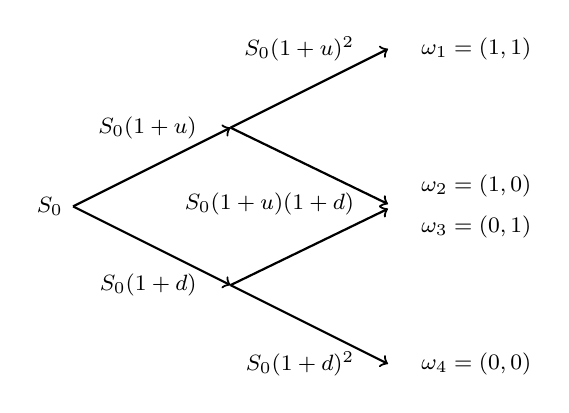
\begin{tikzpicture}
\draw[thick,->] (0,0) node[left] {\footnotesize $S_0$} 
  -- (2,1) node[left,xshift=-3mm] {\footnotesize $S_0(1+u)$};
\draw[thick,->] (0,0) 
  -- (2,-1) node[left,xshift=-3mm] {\footnotesize $S_0(1+d)$};

\draw[thick,->] (2,1) -- (4,2)  
  node[left,xshift=-3mm] {\footnotesize $S_0(1+u)^2$};
\draw[thick,->] (2,1) -- (4,0.03) 
  node[left,xshift=-3mm] {\footnotesize $S_0(1+u)(1+d)$};
\draw[thick,->] (2,-1) -- (4,-0.03);
\draw[thick,->] (2,-1) -- (4,-2) 
  node[left,xshift=-3mm] {\footnotesize $S_0(1+d)^2$};

\draw (4,2) node[xshift=3mm,right] {\footnotesize $\omega_1=(1,1)$};
\draw (4,0) node[xshift=3mm,above right] {\footnotesize $\omega_2=(1,0)$};
\draw (4,0) node[xshift=3mm,below right] {\footnotesize $\omega_3=(0,1)$};
\draw (4,-2) node[xshift=3mm,right] {\footnotesize $\omega_4=(0,0)$};
\end{tikzpicture}
\caption{Дерево для цены рискового актива в двухшаговой модели.}
\label{crr:tree}
\end{figure}

\begin{remark}
Формальное определение цены рискового актива в момент времени $t$ как функции от случайного исхода дается формулой
\[
S_t(\omega) = S_0 (1+u)^{\sum_{i=1}^t a_i} (1+d)^{t-\sum_{i=1}^t a_i}\ \text{для}\ \omega = (a_1,\dots,a_T).
\]
Показатель первой степени здесь равен количеству шагов вверх до момента $t$, а второй "--- количеству шагов вниз.
\end{remark}


\subsection{Торговые стратегии и условие самофинансируемости}

\emph{Торговой стратегией} будем называть последовательность $\pi_t=(G_t,H_t)$, $t=1,\dots,T$, где пара $(G_t,H_t)$ задает портфель активов, который покупается в момент времени $t-1$ и держится до момента $t$.
Величина $G_t$ выражает количество единиц безрискового актива в портфеле, а $H_t$ -- количество единиц рискового. 

Величины $G_t$, $H_t$ могут зависеть от рыночных цен рискового актива или, эквивалентно, от случайного исхода $\omega$.
Таким образом, мы считаем $G_t(\omega)$ и $H_t(\omega)$ случайными величинами, а $\pi_t(\omega)$ случайным вектором.
Как принято в теории вероятностей, указание зависимости от $\omega$ будет для краткости опускаться.

Следует учесть важное обстоятельство: портфель $\pi_t$, будучи купленным в момент $t-1$, не должен зависеть от цены рискового актива в последующие моменты времени.
Это можно сформулировать так: найдутся неслучайные функции $g_t$ и $h_t$ такие, что%
\footnote{Более подробно: $G_t(\omega) = g_t(S_0, S_1(\omega), \dots, S_{t-1}(\omega))$ и аналогично для $H_t$.
В следующей лекции мы узнаем, как можно более лаконично определить такую зависимость через понятие \emph{фильтрации}.}
$G_t=g_t(S_1,\dots,S_{t-1})$ и $H_t=h_t(S_1,\dots,S_{t-1})$.
При $t=1$ величины $G_1$ и $H_1$ не зависят от цен рискового актива и потому представляют собой константы%
\footnote{Заметим, что мы не говорим о зависимости от $S_0$, так как величина $S_0$ считается зафиксированной -- это цена рискового актива на рынке сейчас, она известна и неслучайна.}.

Эквивалентным образом, можно сказать, что случайные величины $G_t$ и $H_t$ должны обладать следующим свойством: для любых исходов $\omega = (a_1,\dots,a_T)$ и $\omega' = (a_1',\dots,a_T')$ таких, что $a_s = a_s'$ для всех $s=1,\dots,t-1$, выполнены равенства $G_t(\omega) = G_t(\omega')$ и $H_t(\omega) = H_t(\omega')$.

\begin{definition}
\emph{Стоимостью портфеля} стратегии $\pi$ в момент $t=1,\dots,T$ будем называть (случайную) величину
\[
V_t^\pi = G_tB_t + H_t S_t,
\]
а в момент $t=0$ (неслучайную) величину
\[
V_0^\pi = G_1 + H_1 S_0.
\]
\end{definition}

Таким образом, под стоимостью портфеля в момент $t$ понимается сумма денег, которую трейдер может выручить в момент времени $t$ от продажи портфеля $\pi_t$, который он купил в момент $t-1$. Так как в момент $t=0$ предыдущего портфеля не было, то мы полагаем $V_0^\pi$ равным стоимости первого портфеля%
\footnote{Может показаться, что здесь есть разногласие между формулами в нулевой момент времени и всеми остальными моментами.
Однако далее мы будем рассматривать только те стратегии, стоимость портфеля которых не меняется в течение торгов (см.~следующее определение). Для них имеет место равенство $V_t^\pi = G_{t+1}B_t + H_{t+1}S_t$ для всех $t=0,\dots,T-1$.}.

Следующее определение вводит важный класс стратегий, у которых нет притока или оттока капитала извне.
Только такие стратегии будут рассматриваться в задаче репликации платежных обязательств при определении их цен.

\begin{definition}
Стратегия $\pi$ называется \emph{самофинансируемой}, если для всех $t=1,\dots,T-1$ выполняется равенство
\begin{equation}
\label{crr:sf}
(H_{t+1} - H_t)S_t = -(G_{t+1} - G_t)B_t.
\end{equation}
\end{definition}
Смысл равенства \eqref{crr:sf} состоит в том, что изменение стоимости позиции по рисковому активу должно в точности покрываться изменением стоимости позиции по безрисковому активу (\te\ купить рисковый актив можно только за счет продажи безрискового, и наоборот). 
Считается, что торговля происходит в моменты $t=0,\dots,T$, причем в течение торгов цены активов остаются зафиксированными, однако они изменяются между моментами торгов. Таким образом, изменение стоимости портфеля может происходить только за счет изменения цен активов, и, следовательно, у самофинансируемой стратегии отсутствует приток или отток капитала.

\begin{remark}
Равенство \eqref{crr:sf} можно также записать в виде
%\begin{equation}
%\label{crr:sf-2}
\[
G_tB_t + H_tS_t = G_{t+1}B_t + H_{t+1}S_t, \qquad t=1,\dots,T-1,
\]
%\end{equation}
что имеет следующий смысл: стоимость портфеля $\pi_t$, с которым мы начинаем торги в момент времени $t$, равна стоимости портфеля $\pi_{t+1}$, с которым мы заканчиваем торги.
Опять-таки, это означает, что нет притока и оттока капитала.
\end{remark}

% Из определения стоимости портфеля и равенства \eqref{crr:sf-2} сразу следует удобная эквивалентная форма условия самофинансируемости: для $t=0,\dots,T-1$ должно быть выполнено равенство
% \begin{equation}
% \label{crr:sf-equiv}
% V_t^\pi = G_{t+1}B_t + H_{t+1}S_t.
% \end{equation}

Докажем одно полезное представление для стоимости портфеля самофинансируемой стратегии, которое далее будет часто использоваться.

\begin{proposition}
\label{crr:p:sf-value}
Для любой самофинансируемой стратегии верно равенство
\begin{equation}
\label{crr:sf-value}
V_t^\pi = V_0^\pi + \sum_{s=1}^t (G_u \Delta B_u + H_u\Delta S_u),
\end{equation}
где $\Delta B_u = B_u - B_{u-1}$, $\Delta S_u = S_u - S_{u-1}$ обозначают изменения цен за период.
\end{proposition}
Интерпретация формулы \eqref{crr:sf-value}: в момент времени $t$ стоимость портфеля самофинансируемой стратегии складывается из начальной стоимости портфеля и суммы изменений стоимости за каждый шаг до момента $t$.
\begin{proof}
Докажем по индукции.
Для $t=0$ утверждение, очевидно, верно.
Если оно верно для $t$, то представим
\begin{multline*}
V_{t+1}^\pi = G_{t+1}B_{t+1} + H_{t+1}S_{t+1} 
= (G_{t+1}B_{t} - G_tB_t + H_{t+1}S_t - H_tS_t)
\\+ (G_tB_t + H_tS_t) + (G_{t+1}\Delta B_{t+1} + H_{t+1}\Delta S_{t+1})
\end{multline*}
(во втором равенство просто добавили и вычли одинаковые слагаемые).
Первая скобка в правой части равна 0 по условию самофинансирования, а вторая скобка равна $V_t^\pi$ по определению стоимости портфеля.
Таким образом,
\[
V_{t+1}^\pi = V_t^\pi + G_{t+1}\Delta B_{t+1} + H_{t+1}\Delta S_{t+1},
\]
откуда следует справедливость шага индукции.
\end{proof}


\subsection{Платежные обязательства}

\begin{definition}
\emph{Платежным обязательством европейского типа} называется контракт между покупателем и продавцом, согласно которому продавец платит покупателю сумму денег $X(\omega)$ в момент времени $T$. 
\end{definition}

Далее все рассматриваемые платежные обязательства будут европейскими, поэтому словосочетание <<европейского типа>> будет опускаться. 


В качестве примера платежных обязательств, можно привести опционы колл и пут с функциями выплат $X^\text{call} = (S_T- K)^+$, $X^\text{put} = (K-S_T)^+$, где $K$ -- цена страйк. Заметим, что выплата $X$ является случайной величиной, причем она может зависеть от всей траектории цены рискового актива, а не только от его цены в последний момент времени.

Нашей следующей задачей будет определить понятие цены платежного обязательства.
Это будет сделано по аналогии с одношаговой моделью: мы покажем, что любое платежное обязательство имеет единственную реплицирующую стратегию, и, следовательно, стоимость портфеля этой стратегии и будет справедливой (безарбитражной) ценой платежного обязательства.


\section{Репликация платежных обязательств}
\subsection{Метод обратной индукции}

В модели КРР цену репликации любого платежного обязательства и реплицирующую стратегию можно найти с помощью \emph{метода обратной индукции}.
Мы сначала сформулируем теорему и рассмотрим конкретный пример, который поможет понять суть доказательства.
Само доказательство приводится в следующем разделе.

\begin{theorem}
В модели КРР для любого платежного обязательства $X$ существует единственная самофинансируемая стратегия $\pi$, называемая \emph{реплицирующей стратегией}, такая, что $V_T^\pi(\omega) = X(\omega)$ для всех $\omega$.
\end{theorem}

\begin{definition}
\emph{Ценой репликации} $V_t^X$ платежного обязательства $X$ в момент времени $t\le T$ называется стоимость портфеля реплицирующей стратегии, \te\ $V_t^X = V_t^\pi$.
\end{definition}

\begin{example}
\label{crr:example}
Рассмотрим двухшаговую модель ($T=2$) с параметрами $S_0=100$, $u=0.1$, $d=-0.1$, $r=0.05$.
Найдем цену репликации опциона колл с временем исполнения $T=2$ и страйком $K=100$.

Будем двигаться назад по моментам времени $t=2,1,0$.
Для $t=2$ цена $V_2^X$ должна равняться $X$, так как если платежное обязательство производит выплату сразу в момент покупки, то его цена равна этой выплате.
Для нашего опциона $X(\omega_1) = 21$ и $X(\omega_i) = 0$, $i=2,3,4$.

В момент $t=1$ имеется две ситуации: цена рискового актива может быть 110 или 90.
В первом случае мы знаем, что в следующий момент времени нам нужно произвести выплату 21 или 0 в зависимости от того, куда пойдет цена.
Из результатов для одношаговой модели, найдем реплицирующий портфель и его стоимость.
Для этого нужно решить систему
\begin{equation}
\label{crr:example-system}
\left\{
\begin{aligned}
&G_2 B_2 + H_2 S_2(\omega_1) = X(\omega_1), \\
&G_2 B_2 + H_2 S_2(\omega_2) = X(\omega_2)
\end{aligned}
\right. \implies
\left\{
\begin{aligned}
&1.05^2 G_2  + 121 H_2 = 21, \\
&1.05^2 G_2 +  99 H_2 = 0.
\end{aligned}
\right.
\end{equation}
Находим $G_2 \approx 85.71$, $H_2 \approx 0.95$ и отсюда получаем стоимость реплицирующего портфеля в момент $t=1$ при цене рискового актива 110: $V_1^X(\omega_1) = V_1^X(\omega_2) = 1.05 G_2 + 110 H_2 = 15$.

Заметим, что если искать компоненты реплицирующей стратегии не требуется, а нужно найти лишь цену репликации, то можно воспользоваться следующей формулой, вытекающей из риск-нейтральной оценки для одношаговой модели:
\begin{equation}
\label{crr:example-step}
V_1(\omega_1) = \frac{21 \cdot q + 0\cdot (1-q)}{1+r} = 15,
\end{equation}
где $q = \frac{r-d}{u-d} = \frac34$ -- риск-нейтральная вероятность. 

Аналогично рассматривается ситуация, когда цена рискового актива в момент $t=1$ равна 90. В этом случае $G_2=H_2 = 0$, $V_1 = 0$ (в следующий момент выплата нулевая).

Наконец, переходим к моменту $t=0$. Нам достаточно построить портфель, который в момент $t=1$ будет стоить $V_1^X$ и в случае, когда цена пойдет вверх, и в случае, когда цена пойдет вниз. 
Если мы найдем такой портфель, то его стоимости будет достаточно, чтобы преобразовать его в уже построенный реплицирующий портфель в момент $t=1$.
Получаем систему, аналогичную \eqref{crr:example-system}:
\[
\left\{
\begin{aligned}
&1.05 G_1  + 110 H_1 = 15, \\
&1.05 G_1 +  90 H_1 = 0.
\end{aligned}
\right.
\]
Решение: $G_1\approx -64.29$, $H_1=3/4$, откуда $V_0^X = G_1 + 100 H_1 \approx 10.71$.
Задача решена.
\end{example}

\begin{remark}
Процесс нахождения цены репликации удобно изображать графически в виде процедуры последовательного заполнения таблицы для значений $V_t$ с конца, см.~рис.~\ref{crr:replication}. 
Сначала нужно составить таблицу цен рискового актива и выплаты опциона (верхняя таблица на рисунке).
Затем положить $V_2=X_2$ (первая таблица во втором ряду). Чтобы найти $V_1$, воспользуемся формулой для риск-нейтральной цены в одношаговой модели (см.~формулу~\eqref{crr:example-step}; в общем случае нужно использовать формулу \eqref{crr:v-by-backward-induction} далее).
Аналогичные вычисления проделываем для $V_0$.

\begin{figure}[h]
\centering
\begin{tabular}{r|ccc|c}
& $S_0$ & $S_1$ & $S_2$ & $X$ \\\hline
$\omega_1$ & 100 & 110 & 121 & 21 \\
$\omega_2$ & 100 & 110 & 99 & 0 \\
$\omega_3$ & 100 & 90 & 99 & 0 \\
$\omega_4$ & 100 & 90 & 81 & 0 \\
\end{tabular}
%
\\[2em]
%
\begin{tabular}{r|ccc}
& $V_0$ & $V_1$ & $V_2$  \\\hline
$\omega_1$ & $\boldsymbol\cdot$ & $\boldsymbol\cdot$  & 21 \\
$\omega_2$ & $\boldsymbol\cdot$ & $\boldsymbol\cdot$  & 0 \\
$\omega_3$ & $\boldsymbol\cdot$ & $\boldsymbol\cdot$  & 0 \\
$\omega_4$ & $\boldsymbol\cdot$ & $\boldsymbol\cdot$  & 0 \\
\end{tabular}
%
$\implies$
%
\begin{tabular}{r|ccc}
& $V_0$ & $V_1$ & $V_2$  \\\hline
$\omega_1$ & $\boldsymbol\cdot$ & 15  & 21 \\
$\omega_2$ & $\boldsymbol\cdot$ & 15  & 0 \\
$\omega_3$ & $\boldsymbol\cdot$ & 0  & 0 \\
$\omega_4$ & $\boldsymbol\cdot$ & 0  & 0 \\
\end{tabular}
%
$\implies$
%
\begin{tabular}{r|ccc}
& $V_0$ & $V_1$ & $V_2$  \\\hline
$\omega_1$ & 10.71 & 15  & 21 \\
$\omega_2$ & 10.71 & 15  & 0 \\
$\omega_3$ & 10.71 & 0  & 0 \\
$\omega_4$ & 10.71 & 0  & 0 \\
\end{tabular}\\[1em]
\caption{Расчет цены опциона с помощью обратной индукции.}
\label{crr:replication}
\end{figure}
\end{remark}


\subsection{\difficult\ Доказательство теоремы}
\textit{Шаг 1 (построение).}
Определим случайные величины $V_t$ для $t=T,\,T-1,\ldots,0$ и $G_t$, $H_t$ для $t=T,\ldots,1$, где $V_t$ будет играть роль цены платежного обязательства или стоимости реплицирующего портфеля, а $G_t$ и $H_t$ "--- роль количества активов в портфеле реплицирующей стратегии.

Для $t=T$ положим $V_T = X$.
Если случайная величина $V_t$ определена, то в качестве $V_{t-1}(\omega)$ для $\omega=(a_1,\dots,a_T)$ возьмем цену репликации в одношаговой биномиальной модели платежного обязательства с выплатой
\[
\tilde X(\omega_u) = V_{t}(a_1,\ldots,a_{t-1}, 1), \qquad
\tilde X(\omega_d) = V_{t}(a_1,\ldots,a_{t-1}, 0),
\]
а значения $G_{t}(\omega)$ и $H_{t}(\omega)$ зададим как решения уравнений 
\begin{equation}
\label{crr:replication-step}
\left\{
\begin{aligned}
&G_t B_t + H_t S_t(a_1,\ldots,a_{t-1}, 1) = V_{t}(a_1,\ldots,a_{t-1}, 1),\\
&G_t B_t + H_t S_t(a_1,\ldots,a_{t-1}, 0) = V_{t}(a_1,\ldots,a_{t-1}, 0).
\end{aligned}
\right.
\end{equation}
Решение системы существует и единственно в силу различия величин $S_t(\ldots, 1)$ и $S_t(\ldots,0)$.
В явном виде имеем
\begin{equation}
\label{crr:v-by-backward-induction}
V_{t-1}(\omega) 
= \frac
  {V_t(a_1,\ldots,a_{t-1}, 1)\cdot q + V_t(a_1,\ldots,a_{t-1}, 0)\cdot (1-q)}
  {1+r} ,
\end{equation}
где $q= \frac{r-d}{u-d}$ -- риск-нейтральная вероятность.
Продолжая по индукции, построим указанные последовательности для всех $t$. 

Отметим, что величины $V_t(\omega)$ зависят только от компонент $a_1,\ldots,a_t$ случайного исхода $\omega=(a_1,\dots,a_T)$, а величины $G_t(\omega)$, $H_t(\omega)$ зависят только от компонент $a_1,\ldots,a_{t-1}$.
В частности, отсюда следует, что последовательность $\pi_t=(G_t,H_t)$ задает торговую стратегию.

\textit{Шаг 2 (проверка).} Покажем, что $V_t^\pi = V_t$, причем $\pi$ является самофинансируемой стратегией и реплицирует $X$.
Заметим, что система \eqref{crr:replication-step} означает равенство
\begin{equation}
\label{crr:replication-value-1}
V_t = G_tB_t + H_t S_t.
\end{equation}
Кроме того, находя в явном виде $G_t$ и $H_t$ и используя \eqref{crr:v-by-backward-induction}, нетрудно проверить, что 
\begin{equation}
\label{crr:replication-value-2}
V_{t-1} = G_tB_{t-1} + H_t S_{t-1}.
\end{equation}
Из равенства \eqref{crr:replication-value-1} следует, что $V_t = V_t^\pi$ для всех $t\ge 1$, а из равенства \eqref{crr:replication-value-2} следует, что $V_0 = V_0^\pi$.
Итак, $V_t^\pi = V_t$ для всех $t=0,\dots,T$.
Из равенств \eqref{crr:replication-value-1} и \eqref{crr:replication-value-2} также нетрудно видеть, что выполнено условие самофинансируемости.
Так как $V_T^\pi = V_T=X$, то $\pi$ реплицирует $X$.

\textit{Шаг 3 (единственность).} Из единственности решения системы \eqref{crr:v-by-backward-induction} следует, что цена репликации определена однозначно.
Тогда единственность реплицирующей стратегии следует из того, если $\pi_t=(G_t,H_t)$ "--- реплицирующая стратегия, то для каждого $t$ и каждого набора $(a_1,\dots,a_{t-1})$ должна быть выполнены равенства
\[
\left\{
\begin{aligned}
&G_t(a_1,\dots,a_{t-1}) B_t + H_t(a_1,\dots,a_{t-1}) S_t(a_1,\ldots,a_{t-1}, 1) = V_{t}(a_1,\ldots,a_{t-1}, 1),\\
&G_t(a_1,\dots,a_{t-1}) B_t + H_t(a_1,\dots,a_{t-1}) S_t(a_1,\ldots,a_{t-1}, 0) = V_{t}(a_1,\ldots,a_{t-1}, 0).
\end{aligned}
\right.
\]
Решение этой системы относительно $G_t,H_t$ единственно.


\section{Риск-нейтральная оценка}

Покажем, что, аналогично одношаговой модели, цены платежных обязательств могут быть вычислены как ожидания дисконтированной выплаты\footnote{Дисконтированной выплатой называется величина $X/B_T$.} по риск-ней\-траль\-ной вероятности. 

Определим риск-нейтральную вероятность в модели КРР по формуле
\[
Q(\omega) = q^{\sum_{i=1}^T a_i} (1-q)^{T-\sum_{i=1}^T a_i}\ \text{для}\ \omega = (a_1,\dots,a_T),
\]
где $q = \frac{r-d}{u-d}$ есть риск-нейтральная вероятность в одношаговой модели.
Таким образом, $Q(\omega)$ приписывает траектории цены рискового актива вероятность пойти вверх на каждом шаге равную $q$ и вероятность пойти вниз $1-q$. 

\begin{example}
Риск-нейтральная вероятность в двухшаговой модели изображена на рис.~\ref{crr:fig:risk-neutral}. Для модели из примера~\ref{crr:example} имеем $q=3/4$, и, следовательно, $Q(\omega_1)=q^2 = 9/16$, $Q(\omega_2)=Q(\omega_3)=q(1-q) = 3/16$, $Q(\omega_4)=(1-q)^2 = 1/16$.

\begin{figure}[h]
\centering
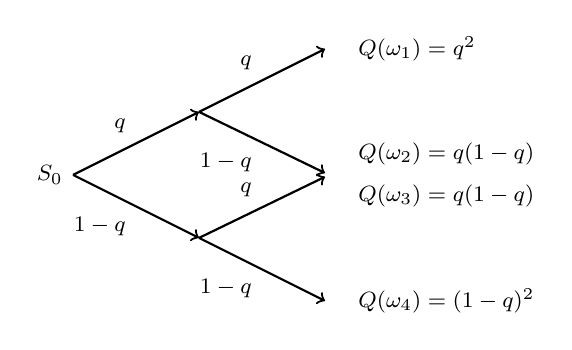
\begin{tikzpicture}[scale=0.8]
\draw[thick,->] (0,0) node[left] {\footnotesize $S_0$} 
  --node[midway,above left] {\footnotesize $q$} (2,1);
\draw[thick,->] (0,0) 
  --node[midway,below left] {\footnotesize $1-q$} (2,-1);

\draw[thick,->] (2,1) --node[midway,above left] {\footnotesize $q$} (4,2);
\draw[thick,->] (2,1) -- node[midway,below left] {\footnotesize $1-q$} (4,0.03);
\draw[thick,->] (2,-1) --node[midway,above left] {\footnotesize $q$} (4,-0.03);
\draw[thick,->] (2,-1) --node[midway,below left] {\footnotesize $1-q$} (4,-2);

\draw (4,2) node[xshift=3mm,right] {\footnotesize $Q(\omega_1)=q^2$};
\draw (4,0) node[xshift=3mm,above right] {\footnotesize $Q(\omega_2)=q(1-q)$};
\draw (4,0) node[xshift=3mm,below right] {\footnotesize $Q(\omega_3)=q(1-q)$};
\draw (4,-2) node[xshift=3mm,right] {\footnotesize $Q(\omega_4)=(1-q)^2$};
\end{tikzpicture}
\caption{Риск-нейтральная вероятность в двухшаговой модели.}
\label{crr:fig:risk-neutral}
\end{figure}
\end{example}

\begin{theorem}
Для цены репликации платежного обязательства $X$ в начальный момент времени%
\footnote{Аналогичная формула будет верна и для цены в промежуточные моменты времени, но чтобы ее записать, нам потребуется понятие условного математического ожидания.
Мы изучим его в следующей лекции.} справедлива формула
\[
V_0^X = \E^Q\left(\frac{X}{B_T}\right) \qquad \left(\;= (1+r)^{-T} \E^Q X\right).
\]
\end{theorem}

\begin{proof}[Доказательство \difficult]
Воспользуемся индукцией по количеству периодов $T$.
Для $T=1$ утверждение верно из результатов для одношаговой модели. 

Пусть $\Omega'$ и $Q'$ обозначают пространство случайных исходов и риск"=нейтральную вероятность в модели с $T-1$ периодами. 
Так как реплицирующая стратегия для $X$ также может реплицировать платежное обязательство с выплатой $X'=V_{T-1}^X$ в момент $T-1$, то из предположения индукции имеем
\[
V_0^X = \E^{Q'}\left(\frac{V_{T-1}^X}{B_{T-1}}\right).
\]
Из риск-нейтральной оценки для одношаговой модели находим
\[
V_{T-1}^X(\omega') = \frac{1}{1+r}(q X(\omega_u') + (1-q) X(\omega_d')),
\]
где $\omega' = (a_1,\ldots,a_{T-1})$ и $\omega'_u = (a_1,\ldots,a_{T-1},1)$, $\omega'_d = (a_1,\ldots,a_{T-1},0)$.
Теперь доказываемое утверждение следует из цепочки равенств
\begin{multline*}
V_0^X = \sum_{\omega'\in\Omega'} 
  \frac{V_{T-1}^X(\omega')}{{B_{T-1}}} Q'(\omega') \\
= \sum_{\omega'\in\Omega'} \frac{1}{(1+r)B_{T-1}}
  \left(X(\omega'_u) q Q'(\omega') + X(\omega'_d) (1-q) Q'(\omega')\right) \\
=  \sum_{\omega\in\Omega} \frac{1}{B_T} X(\omega) Q(\omega) 
= \E^Q\left(\frac{X}{B_T}\right),
\end{multline*}
где во втором равенстве воспользовались тем, что сумму по $\omega'\in \Omega'$ во второй строке можно разбить на две (в одной будут слагаемые с $X(\omega'_u)$, а в другой с $X(\omega'_d)$), а затем перегруппировать слагаемые таким образом, чтобы получить одну сумму по $\omega\in\Omega$.
\end{proof}

\begin{corollary}
\label{crr:martingale}
Для любого $t$ справедливо равенство $S_0 = (1+r)^{-t}\E^Q S_t$.
\end{corollary}
\begin{proof}
Платежное обязательство с выплатой $X=S_t$ в момент $t$ реплицируется портфелем из одной акции (\te\ $\pi_t\equiv(0,1))$, стоимость которого в начальный момент времени равна $S_0$.
С другой стороны, эта же стоимость является ценой репликации, которая по теореме равна $(1+r)^{-t}\E^Q S_t$.
\end{proof}


\section{Примеры оценки платежных обязательств}

\subsection{Бескупонная облигация}
Бескупонная облигация с временем погашения $T$ соответствует платежному обязательству с константой выплатой $X$ (\emph{номиналом} облигации) в момент $T$.
Ее цена задается формулой
\[
V_t^X = (1+r)^{t-T}X.
\]
Это выражение следует из того, что такая облигация реплицируется постоянным портфелем $\pi_t\equiv(G,0)$ с $G = (1+r)^{-T} X$.
Для $t=0$, мы также можем воспользоваться риск-нейтральной оценкой: $V_0^X = (1+r)^{-T} \E^Q X = (1+r)^{-T} X$.

\subsection{Форвардная цена}
\emph{Форвардной ценой} (более точно, $T$-форвардной ценой) рискового актива в момент времени $t=0$ называется (неслучайная) величина $F$ такая, что контракт на покупку актива по цене $F$ в момент времени $t=T$ имеет нулевую стоимость в момент $t=0$. 

Рассматривая платежное обязательство $X=S_T-F$ и приравнивая $V^X_0 = 0$, получаем уравнение
$(1+r)^{-T} \E^Q (S_T - F) = 0$.
Пользуясь следствием~\ref{crr:martingale}, находим $F= (1+r)^T S_0$.

Этот результат можно получить и с помощью репликации.
Действительно, выплата $X=S_T-F$ реплицируется портфелем из одной акции и минус одной бескупонной облигации с номиналом $F$.
В начальный момент стоимость такого портфеля равна $S_0 - (1+r)^{-T} F$.
Нулевую стоимость дает $F = (1+r)^T S_0$.

\subsection{Платежные обязательства, не зависящие от траектории цены}
Если платежное обязательство $X = f(S_T)$ зависит только от цены рискового актива в последний момент времени (как, например, у ванильных опционов), то можно воспользоваться тем, что $S_T$ представима в виде
\[
S_T = S_0 (1+u)^\xi(1+d)^{T-\xi},
\]
где величина $\xi$ равна количеству шагов цены вверх на всей траектории.
Относительно риск-нейтральной вероятности $\xi$ имеет биномиальное распределение с параметрами $T$ и $q$.
Тогда цену репликации можно записать в виде ожидания по биномиальному распределению, что дает формулу
\[
V_0^X = (1+r)^{-T} \sum_{n=0}^T f\left(S_0 (1+u)^n(1+d)^{T-n}\right) \cdot C_T^n q^n (1-q)^{T-n}.
\]

\subsection{Платежные обязательства, зависящие от траектории цены}
Если выплата зависит от всей траектории цены, то воспользоваться формулой с биномиальным распределением не получится, и нужно явно найти риск-нейтральную вероятность каждой траектории и выплату на этой траектории.

\begin{example}
\label{crr:e:barrier}
Рассмотрим двухшаговую модель с параметрами из примера \ref{crr:example} и вычислим в ней цену \emph{барьерного опциона вниз-и-выход} колл с со страйком $K=95$ и барьером $H=92$. Этот опцион разрешается исполнить только если его цена за все моменты времени не опустится ниже $H$.
Выплата имеет следующий вид
\[
X(\omega_1) = 26, \quad X(\omega_2) = 4, \quad X(\omega_3) = X(\omega_4)=0.
\]
Используя риск-нейтральные вероятности исходов из примера \ref{crr:example}, получаем
\[
V_0^X = \frac1{1.05^2}\left(26 \cdot \frac9{16} + 4\cdot \frac3{16}\right) \approx 13.95.
\]
\end{example}

\begin{remark}
К сожалению, подобный метод вычисления становится слишком трудоемким при увеличении числа шагов в модели, так как число траекторий растет экспоненциально.
Тем не менее, часто получается упростить задачу, если выплата $X$ задается функцией от некоторой  случайной последовательности, обладающей марковским свойством (но мы не будем касаться этого подхода). 

Другой способ заключается в симуляции траекторий моделей и вычислении математического ожидания в формуле для цены платежного обязательства с помощью метода Монте-Карло.
Мы подробно рассмотрим метод Монте-Карло для модели \bs\ в лекции \ref{ch:mc}; большинство рассуждений оттуда можно перенести и на модель \crr.
\end{remark}

\subsection{Паритет цен колл"--~пут}
Аналогично одношаговой биномиальной модели, в модели КРР справедливо равенство 
\[
C-P = S_0 - \frac{K}{B_T} \quad (= S_0 - K(1+r)^{-T}),
\]
где $C$ и $P$ "--- цены (в момент времени 0) европейских опционов колл и пут со одинаковым страйком $K$ и временем исполнения $T$.
Доказательство аналогично формуле \eqref{os:parity-proof} в лекции \ref{ch:onestep}:
\[
C - P = \E^Q \frac{(S_T-K)^+ - (K-S_T)^+ }{B_T}
= \E^Q \frac{S_T - K}{B_T} = S_0 - \frac{K}{B_T}.
\]
Можно также дать доказательство через репликацию выплаты длинной позиции по опциону колл и короткой позиции по опциону пут с помощью бескупонной облигации и рискового актива (упражнение). 


\summary

\begin{itemize}
\item В модели \crr\ (многошаговой биномиальной модели) безрисковый актив имеет цену $B_t=(1+r)^t$, а цена рискового актива на каждом шаге может изменяться в $1+u$ или $1+d$ раз, где $d<r<u$.

\item Любое платежное обязательство $X$ реплицируемо.
Реплицирующую стратегию можно найти методом обратной индукции.
Цену репликации в момент $t=0$ можно найти по формуле
\[
V^X_0 = \E^{\Q} \frac{X}{B_T},
\]
где $\Q$ "--- риск-нейтральная вероятность, относительно которой цена рискового актива идет вверх с вероятностью $q_u = \frac{r-d}{u-d}$ и вниз с вероятностью $q_d = \frac{u-r}{u-d}$.

\item Цена бескупонной облигации с номиналом $X$: $B = X/(1+r)^T$.

\item Форвардная цена рискового актива: $F=(1+r)^TS_0$.

\item Паритет цен пут"--~колл: $C-P = S_0 - K/B_T$.
\end{itemize}
